\documentclass{standalone}

\usepackage{tikz}
\usetikzlibrary{calc,shapes.multipart,chains,arrows,positioning}
\tikzset{
    squarecross/.style={
        draw, rectangle,minimum size=18pt, fill=orange!80,
        inner sep=0pt, text=black,
        path picture = {
            \draw[black]
            (path picture bounding box.north west) -- 
            (path picture bounding box.south east)
            (path picture bounding box.south west) -- 
            (path picture bounding box.north east);
        }
    }
}

\begin{document}
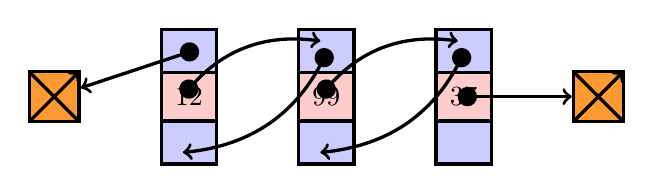
\begin{tikzpicture}[
        list/.style={
            very thick, rectangle split, 
            rectangle split parts=3, draw, 
            minimum size=18pt,
            inner sep=5pt, text=black,
            rectangle split part fill={blue!20, red!20, blue!20}
        }, 
        ->, start chain, very thick
      ]

  \node[list,on chain] (A) {\nodepart{second} 12};
  \node[list,on chain] (B) {\nodepart{second} 99};
  \node[list,on chain] (C) {\nodepart{second} 37};

  \node[squarecross]   (D) [right=of C] {};
  \node[squarecross]   (E) [left= of A] {};

  \path[*->] let \p1 = (A.three), \p2 = (A.center) in (\x1,\y2) edge [bend left] ($(B.one)+(0,0.2)$);
  \path[*->] let \p1 = (B.three), \p2 = (B.center) in (\x1,\y2) edge [bend left] ($(C.one)+(0,0.2)$);
  \draw[*->] let \p1 = (C.three), \p2 = (C.center) in (\x1,\y2) -- (D);

  \draw[*->] ($(A.one)+(0.2,0.1)$) -- (E);
  \path[*->] ($(B.one)+(0.1,0.1)$) edge [bend left] ($(A.three)+(0,-0.05)$);
  \path[*->] ($(C.one)+(0.1,0.1)$) edge [bend left] ($(B.three)+(0,-0.05)$);

\end{tikzpicture}
\end{document}